\documentclass[11pt]{article} 

% packages with special commands
\usepackage{amssymb, amsmath}
\usepackage{epsfig}
\usepackage{array}
\usepackage{ifthen}
\usepackage{color}
\usepackage{fancyhdr}
\usepackage{graphicx}
\usepackage{mathtools}
%\usepackage{algorithm}
%\usepackage{algpseudocode}
%\usepackage{mdframed}
%\newmdtheoremenv{lem}{Lemma}
\definecolor{grey}{rgb}{0.5,0.5,0.5}

\begin{document}
\newcommand{\tr}{\text{tr}}
\newcommand{\E}{\textbf{E}}
\newcommand{\diag}{\text{diag}}
\newcommand{\argmax}{\text{argmax}}
\newcommand{\Cov}{\text{Cov}}
\newcommand{\Var}{\text{Var}}
\renewcommand{\thefootnote}{\fnsymbol{footnote}}

\begin{center}
\noindent Charles Zheng EE 378b HW 4
\end{center}

\noindent\textbf{1.}
We use the following procedure for all three.
\begin{enumerate}
\item Find $v$, the first eigenvector for ${A-D , D^{-1/2}AD^{-1/2}-I, B}$
\item Search over values $c$: compute the modularity of the partition $\{i: v_i > c\} \cup \{i: v_i \leq c\}$.  Limit this search to values for $c$ producing partitions with at least 20 nodes.
\item If the modularity of the best obtained partition exceeds the modularity of the entire graph, partition the graph and apply the procedure to each of the two subgraphs obtained.  Otherwise, stop.
\end{enumerate}

The results are as follows:
\begin{tabular}{c|c|c}
Matrix & No. clusters & Modularity \\ \hline
$A - D$ & 6 & 7415.6\\
$D^{-1/2}AD^{-1/2}-I$ & 47 & 1413.2\\
$B$ & 75 & 17205.1
\end{tabular}

The modularity matrix $B$ gives the best result by far, while the normalized Lapalcian is seen to be quite ill-suited for this problem.

\noindent\textbf{2.}
All of the 10 initializations converged (reached a local minimum) within $10n$ iterations.

\begin{center}
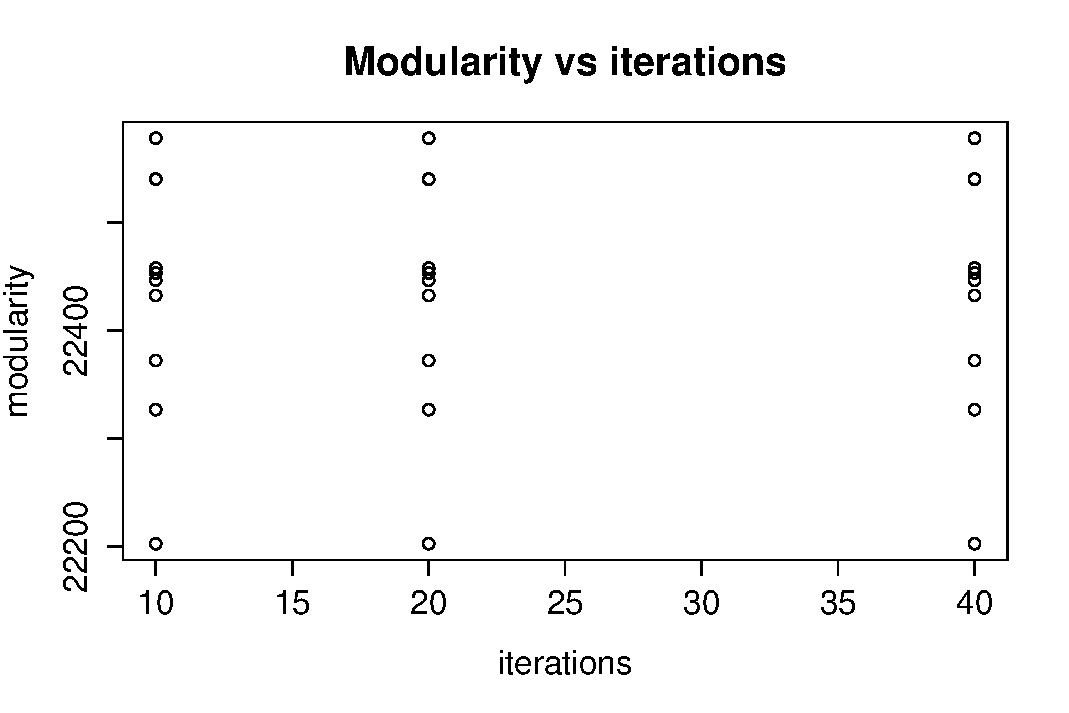
\includegraphics[scale=0.3]{figure/hw2_2.pdf}
\end{center}

The maximum modularity obtained was 22578.2, which exceeds the best obtained in step 1.

\noindent\textbf{3.}

We initialize the greedy algorithm with the clusters from step 1.

\begin{tabular}{c|c|c}
Matrix & No. clusters & Modularity \\ \hline
$A - D$ & 6 & 19038.8\\
$D^{-1/2}AD^{-1/2}-I$ & 47 & 20749.8\\
$B$ & 75 & 23328.1
\end{tabular}

In all cases the modularity increased substantially, and by using the cluster obtained from the modularity matrix $B$ we can do better than the random initializations in part 2.


\end{document}
